% Procédure du projet A1 (filtrage collaboratif), groupe 40 « La piscine ».
% Compilation (depuis docs/procedure/) : latexmk -pdf procedure.tex
% Les figures sont lues dans ../../figures/ (produites par experiments/*.py).
\documentclass[11pt,a4paper]{article}

\usepackage[T1]{fontenc}
\usepackage[utf8]{inputenc}
\usepackage[french]{babel}
\usepackage{lmodern}
\usepackage{microtype}
\usepackage{amsmath,amssymb}
\usepackage{booktabs}
\usepackage{graphicx}
\usepackage{xcolor}
\usepackage{enumitem}
\usepackage[margin=2.4cm]{geometry}
\usepackage{caption}
\usepackage{float}
\usepackage[most]{tcolorbox}
\usepackage[hidelinks]{hyperref}

\graphicspath{{../../figures/}}

\definecolor{accent}{HTML}{2A6FDB}
\definecolor{warm}{HTML}{E8833A}
\definecolor{ok}{HTML}{1A9E5C}

\setlist{itemsep=2pt, topsep=4pt}
\setlength{\parskip}{4pt}
\setlength{\parindent}{0pt}

% Bloc « étape » : titre, objectif, livrable.
\newtcolorbox{etape}[1]{enhanced, breakable, colback=accent!4, colframe=accent,
  boxrule=0.6pt, arc=2pt, left=8pt, right=8pt, top=6pt, bottom=6pt,
  fonttitle=\bfseries, title={#1}}
% Encadré « à retenir ».
\newtcolorbox{retenir}{enhanced, colback=warm!7, colframe=warm, boxrule=0.6pt,
  arc=2pt, left=8pt, right=8pt, fonttitle=\bfseries, title={À retenir}}

\newcommand{\R}{\mathbb{R}}
\newcommand{\rhat}{\hat r}

\title{\textbf{Projet A1 --- Filtrage collaboratif}\\[4pt]
  \large Procédure, méthodes et feuille de route}
\author{Groupe 40 \og La piscine \fg{} --- DataLab, Master IASD}
\date{11 octobre 2026}

\begin{document}
\maketitle

\begin{abstract}
\noindent Ce document fixe ce que nous devons rendre, comment nous mesurons nos
résultats et dans quel ordre nous implémentons les méthodes. Il sert de fil
conducteur commun pour le code, les slides du 14 octobre et le rapport du
21 octobre. Les chiffres cités sont ceux de nos premières expériences
(entraînement sur \texttt{ratings\_train}, score sur \texttt{ratings\_test}).
\end{abstract}

\tableofcontents
\newpage

%=============================================================================
\section{Le problème et les règles du jeu}
%=============================================================================

\subsection{La tâche}

On dispose d'une matrice de notes $R \in \R^{n \times m}$ avec $n = 610$
utilisateurs et $m = 4980$ films (copie de MovieLens). Les notes vont de $0{,}5$ à
$5$ par pas de $0{,}5$ et seule une petite fraction des cases est connue. Il faut
\textbf{prédire toutes les cases manquantes} : le script \texttt{generate.py}
lit une matrice incomplète et écrit la matrice complétée dans
\texttt{output.npy}.

La qualité est mesurée par la RMSE sur un ensemble $T$ de notes cachées :
\[
  \mathrm{RMSE} = \sqrt{\frac{1}{|T|} \sum_{(u,i) \in T} \bigl(r_{ui} - \rhat_{ui}\bigr)^2 } .
\]
La plateforme affiche aussi l'\emph{accuracy} (proportion de notes exactes après
arrondi au demi-point) et le temps d'exécution.

\subsection{Trois jeux de données, deux protocoles}

Les notes sont réparties en trois paquets disjoints : \emph{train} et \emph{test}
nous sont donnés, \emph{eval} est gardé par l'enseignant.

\begin{table}[H]
\centering
\begin{tabular}{@{}lll@{}}
\toprule
 & \textbf{Entrée du modèle} & \textbf{Score calculé sur} \\
\midrule
Nos expériences locales & train (31\,598 notes) & test (31\,598 notes) \\
La plateforme           & train + test (63\,196 notes) & eval (caché) \\
\bottomrule
\end{tabular}
\end{table}

La plateforme voit donc \textbf{deux fois plus de notes} que nos expériences :
les scores du classement seront meilleurs que nos scores locaux, et les
hyperparamètres optimaux peuvent légèrement bouger (moins de régularisation,
rang un peu plus grand).

\subsection{Contraintes et échéances}

\begin{itemize}
  \item \textbf{Calcul :} 1200\,s au maximum, 4 threads CPU, 12\,Go de mémoire,
        pas de GPU. Le dépôt est testé chaque matin vers 5\,h.
  \item \textbf{Interface :} ne pas modifier les lignes de chargement et de
        sauvegarde de \texttt{generate.py} ; lister les dépendances dans
        \texttt{requirements.txt}.
  \item \textbf{Évaluation :} le code n'est pas noté. Seuls comptent le rapport et
        la présentation : protocole, résultats, interprétation, limites.
\end{itemize}

\begin{table}[H]
\centering
\begin{tabular}{@{}ll@{}}
\toprule
\textbf{Date} & \textbf{Échéance} \\
\midrule
14 oct., 23:59 & \texttt{slides.pdf} à la racine du dépôt (notre groupe présente le 15) \\
15 oct.        & Présentation préliminaire : \textbf{5 minutes exactement} \\
21 oct., 23:59 & \texttt{report.pdf} : page de garde + 5 pages au maximum \\
22 oct., 05:00 & Dernière version du code prise en compte \\
\bottomrule
\end{tabular}
\end{table}

\begin{retenir}
Le travail attendu (slide 34 du cours) tient en quatre points :
\begin{enumerate}[label=\arabic*.]
  \item une factorisation de matrice entraînée par \textbf{ALS ou descente de gradient} ;
  \item au moins \textbf{une approche alternative} ;
  \item une \textbf{comparaison à une baseline} avec un protocole clair ;
  \item une discussion des \textbf{hyperparamètres, de la régularisation, des
        découpages et du coût de calcul}.
\end{enumerate}
Aucun retard n'est accepté ; un fichier mal nommé est pénalisé.
\end{retenir}

%=============================================================================
\section{Ce que disent les données}
%=============================================================================

Avant de choisir une méthode, trois constats orientent tout le reste.

\paragraph{1. La matrice est extrêmement creuse.} Seules $1{,}04\,\%$ des cases
sont remplies en train. Un film reçoit en médiane \textbf{3 notes}, et $65\,\%$
des films en ont moins de 5. Côté utilisateurs, la médiane est de 24 notes. Le
volume est très concentré : $10\,\%$ des films réunissent $46\,\%$ des notes
(figure~\ref{fig:eda}, gauche).

\paragraph{2. Les biais expliquent l'essentiel.} Certains utilisateurs notent
systématiquement haut, certains films sont systématiquement bien notés. Le seul
modèle $\mu + b_u + b_i$ fait passer la RMSE de $1{,}037$ (moyenne globale) à
$0{,}875$.

\paragraph{3. Au-delà des biais, le signal est faible.} Une fois les biais
retirés, le spectre de la matrice des résidus se confond avec celui d'une
matrice de bruit de même structure au-delà du rang~5 environ
(figure~\ref{fig:eda}, droite). On doit donc s'attendre à des \textbf{rangs
faibles} et à une \textbf{régularisation forte}.

\begin{figure}[H]
\centering
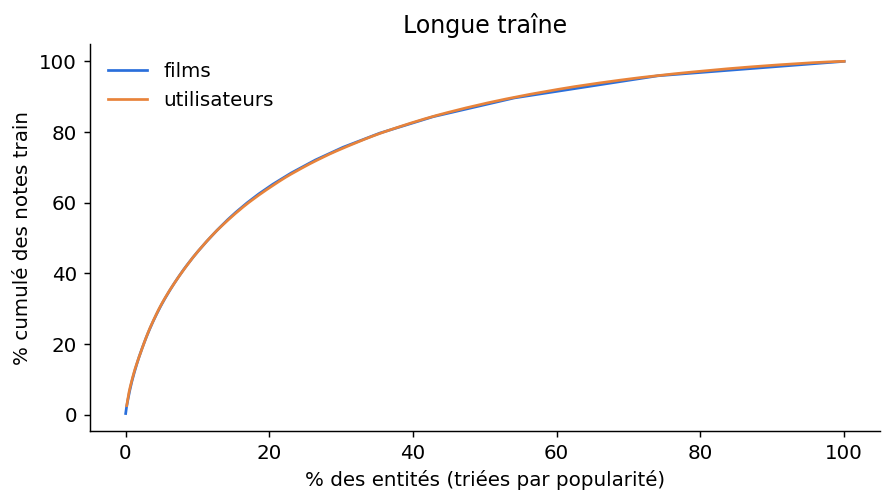
\includegraphics[width=0.42\linewidth]{eda/03_long_tail.png}\hfill
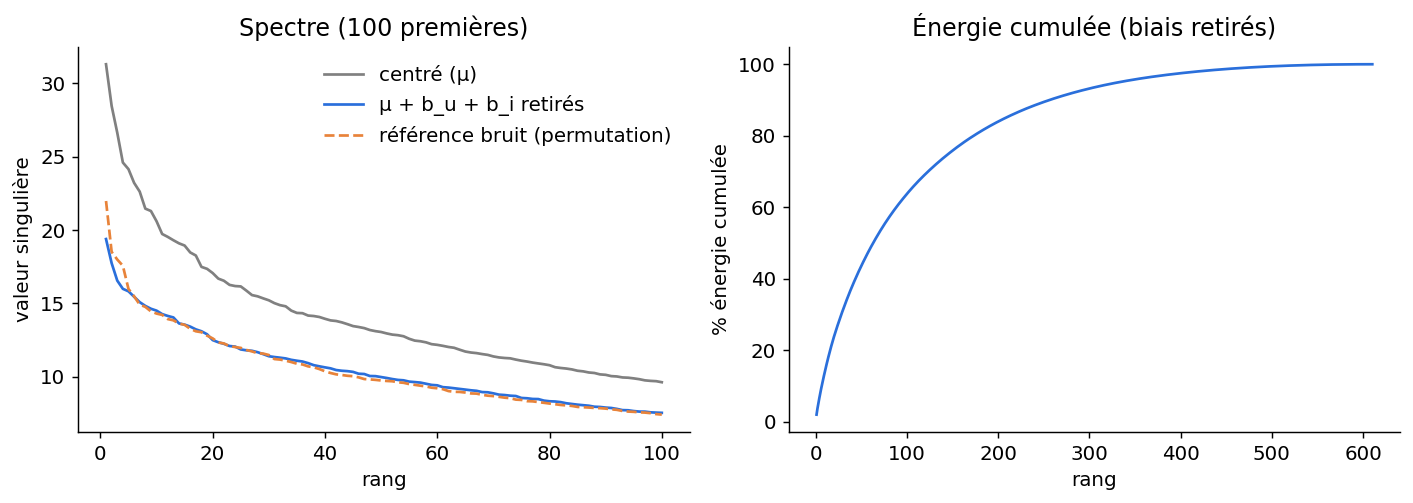
\includegraphics[width=0.56\linewidth]{eda/10_svd_spectrum.png}
\caption{Gauche : longue traîne des notes. Droite : spectre des résidus après
retrait des biais (bleu) comparé à une référence de bruit obtenue par
permutation (orange pointillé).}
\label{fig:eda}
\end{figure}

Il n'y a pas de vrai démarrage à froid : tout utilisateur et tout film du test a
au moins une note en train. Mais $21\,\%$ des notes de test portent sur un film
qui a moins de 5 notes en train : c'est là que se jouent les plus grosses
erreurs. Les genres et l'année (fichier \texttt{namesngenre.npy}) ont un effet
direct faible (environ $\pm 0{,}15$ sur la note moyenne), mais peuvent aider ces
films peu notés.

%=============================================================================
\section{Protocole expérimental}
%=============================================================================

Toutes les méthodes suivent la même procédure, pour que les comparaisons soient
honnêtes.

\begin{enumerate}[label=\textbf{\arabic*.}]
  \item \textbf{Réglage.} On tire au hasard $10\,\%$ des notes de train
        (graine~0) comme ensemble de validation. Chaque configuration
        d'hyperparamètres est entraînée sur les $90\,\%$ restants et notée sur
        la validation.
  \item \textbf{Score final.} La meilleure configuration est réentraînée sur
        tout le train, puis évaluée \textbf{une seule fois} sur le test. Le test
        ne sert jamais à choisir quoi que ce soit.
  \item \textbf{Mesures.} RMSE (critère principal), accuracy après arrondi au
        demi-point, temps d'entraînement. Les prédictions sont ramenées dans
        $[0{,}5\,;\,5]$.
  \item \textbf{Analyse fine.} On découpe la RMSE de test selon le nombre de
        notes du film en train, pour voir \emph{où} chaque méthode aide.
\end{enumerate}

Dans le code, chaque modèle expose la même interface :
\texttt{fit\_xxx(train, shape, **hp)} renvoie une fonction
\texttt{predict(u, i)}. Les scripts \texttt{experiments/run\_*.py} rejouent
toutes les expériences et écrivent les résultats dans \texttt{results/} et les
figures dans \texttt{figures/}.

%=============================================================================
\section{Feuille de route : les étapes dans l'ordre}
%=============================================================================

Les étapes sont ordonnées pour que chacune serve de référence à la suivante.
Les étapes 0 à 4 sont faites ; la présentation du 15 octobre s'appuie dessus.

%-----------------------------------------------------------------------------
\begin{etape}{Étape 0 --- Un premier rendu valide sur la plateforme \hfill \textcolor{ok}{fait}}
\textbf{Objectif :} vérifier toute la chaîne (dépendances, interface, temps) et
obtenir un premier score officiel.

\textbf{Réalisé :} \texttt{generate.py} produit les biais régularisés en
$0{,}4$\,s. RMSE locale : $0{,}8746$ (contre $1{,}037$ pour le code de départ).
\end{etape}

%-----------------------------------------------------------------------------
\begin{etape}{Étape 1 --- Baselines \hfill \textcolor{ok}{fait}}
\textbf{Objectif :} fixer le point de comparaison de toutes les méthodes.

\textbf{Modèle :} $\rhat_{ui} = \mu + b_u + b_i$, avec des biais régularisés
\[
  \min_{b} \sum_{(u,i)\,\text{observés}} \bigl(r_{ui} - \mu - b_u - b_i\bigr)^2
  + \lambda \Bigl(\sum_u b_u^2 + \sum_i b_i^2\Bigr).
\]
On alterne les deux mises à jour en forme fermée :
$b_i = \frac{\sum_{u} (r_{ui} - \mu - b_u)}{\lambda + n_i}$ et symétriquement
pour $b_u$. Le terme $\lambda$ tire vers 0 les biais des films peu notés.

\textbf{Résultat :} $\lambda = 2$ donne $0{,}8746$. Sans régularisation, on
monte à $0{,}919$ : la régularisation est indispensable dès cette étape.
\end{etape}

%-----------------------------------------------------------------------------
\begin{etape}{Étape 2 --- Factorisation de matrice (exigée) \hfill \textcolor{ok}{fait, à affiner}}
\textbf{Objectif :} implémenter la méthode centrale du cours et étudier rang,
régularisation et coût.

\textbf{Modèle :} on ajoute aux biais un produit de facteurs latents de rang $k$,
\[
  \rhat_{ui} = \mu + b_u + b_i + p_u^\top q_i, \qquad p_u, q_i \in \R^k,
\]
appris en minimisant l'erreur \emph{sur les seules notes observées} :
\[
  \sum_{(u,i)\,\text{observés}} \bigl(r_{ui} - \rhat_{ui}\bigr)^2
  + \lambda_f \bigl(\|P\|_F^2 + \|Q\|_F^2\bigr)
  + \lambda_b \bigl(\|b_u\|^2 + \|b_i\|^2\bigr).
\]

\textbf{Deux optimiseurs, comme dans le cours :}
\begin{itemize}
  \item \textbf{ALS.} Le coût est convexe en $P$ quand $Q$ est fixé, et
        inversement. Chaque $p_u$ est la solution d'une petite régression ridge
        sur les films notés par $u$ :
        $p_u = \bigl(Q_u^\top Q_u + \lambda_f I\bigr)^{-1} Q_u^\top \tilde r_u$,
        où $\tilde r_u$ sont les notes de $u$ sans les biais. On alterne
        utilisateurs et films.
  \item \textbf{Descente de gradient stochastique (SGD).} Pour chaque note,
        $e_{ui} = r_{ui} - \rhat_{ui}$, puis
        $p_u \leftarrow p_u + \eta\,(e_{ui}\, q_i - \lambda_f\, p_u)$ et
        symétriquement pour $q_i$ et les biais.
\end{itemize}

\textbf{Choix importants :} deux régularisations séparées, $\lambda_b$ pour les
biais et $\lambda_f$ pour les facteurs. Avec un seul $\lambda$, soit les biais
sont trop contraints, soit les facteurs surapprennent. Option ALS-WR : pénalité
proportionnelle au nombre de notes de chaque ligne.

\textbf{À montrer :} courbes de RMSE train/validation au fil des itérations
(sans régularisation, la validation remonte : surapprentissage), RMSE selon le
rang pour plusieurs $\lambda_f$, coût en temps.

\textbf{Résultats} (180 configurations ALS, 48 SGD, choisies sur la validation) :
\begin{itemize}
  \item ALS, $k = 20$, $\lambda_f = 10$, $\lambda_b = 2$ : \textbf{0,8725} en $1{,}5$\,s ;
  \item ALS-WR, $k = 20$ : meilleur en validation (0,8874) mais 0,8746 en test ;
  \item SGD, $k = 20$, arrêt précoce à 17 époques : 0,8775 en $0{,}5$\,s.
\end{itemize}
Le gain sur les biais est réel mais faible, conformément au spectre de la
figure~\ref{fig:eda}. Sans régularisation, l'erreur d'entraînement tombe à 0
et la validation dépasse 1,0 (figure~\ref{fig:mf}). Avec $\lambda_f \geq 15$,
les facteurs s'annulent et on retrouve exactement les biais : la fenêtre utile
est étroite. Une fois $\lambda_f$ bien réglé, le rang compte peu.

\textbf{Détail technique :} sous Windows, résoudre 5\,000 petits systèmes
linéaires d'un coup avec \texttt{numpy} était 100 fois plus lent qu'avec
\texttt{torch.linalg.solve}, à cause du multithreading d'OpenBLAS. Une
itération d'ALS est passée de 17\,s à $0{,}1$\,s.
\end{etape}

\begin{figure}[H]
\centering
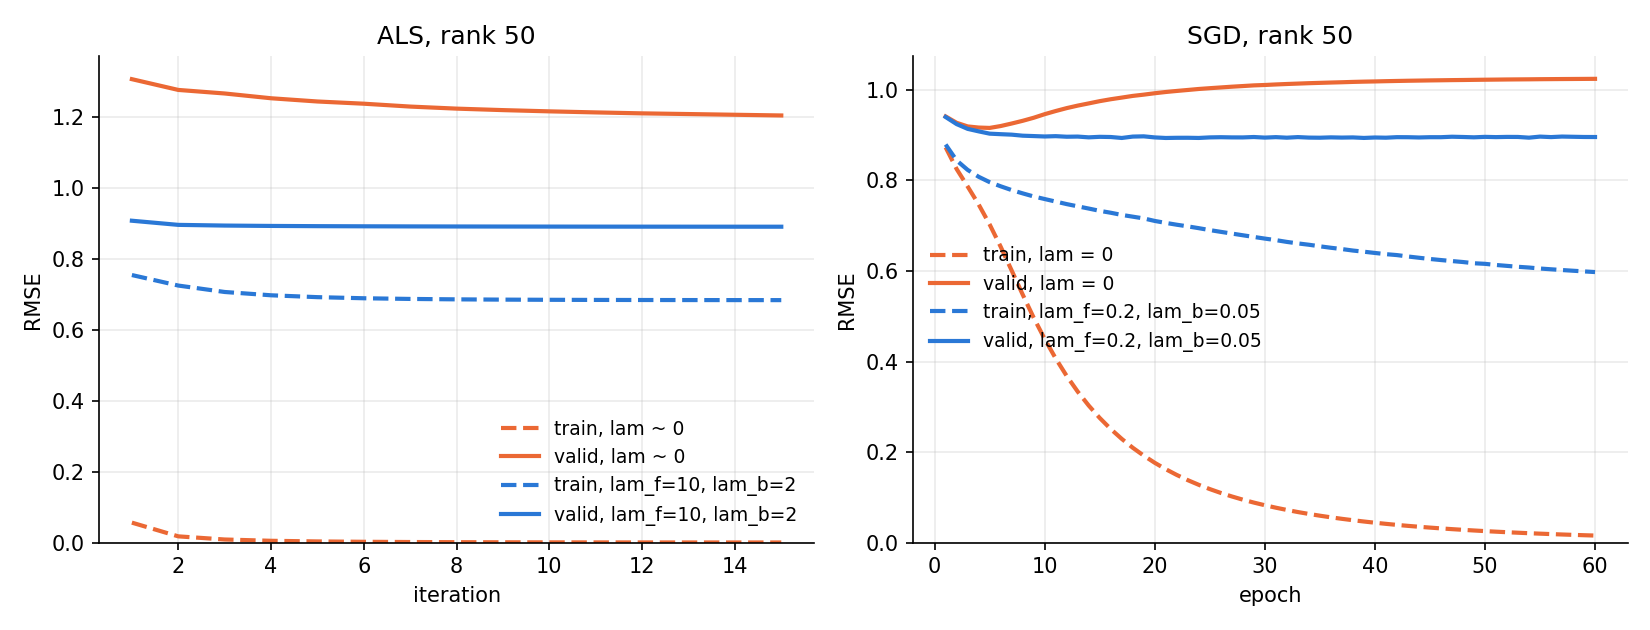
\includegraphics[width=0.8\linewidth]{mf_learning_curves.png}\\[4pt]
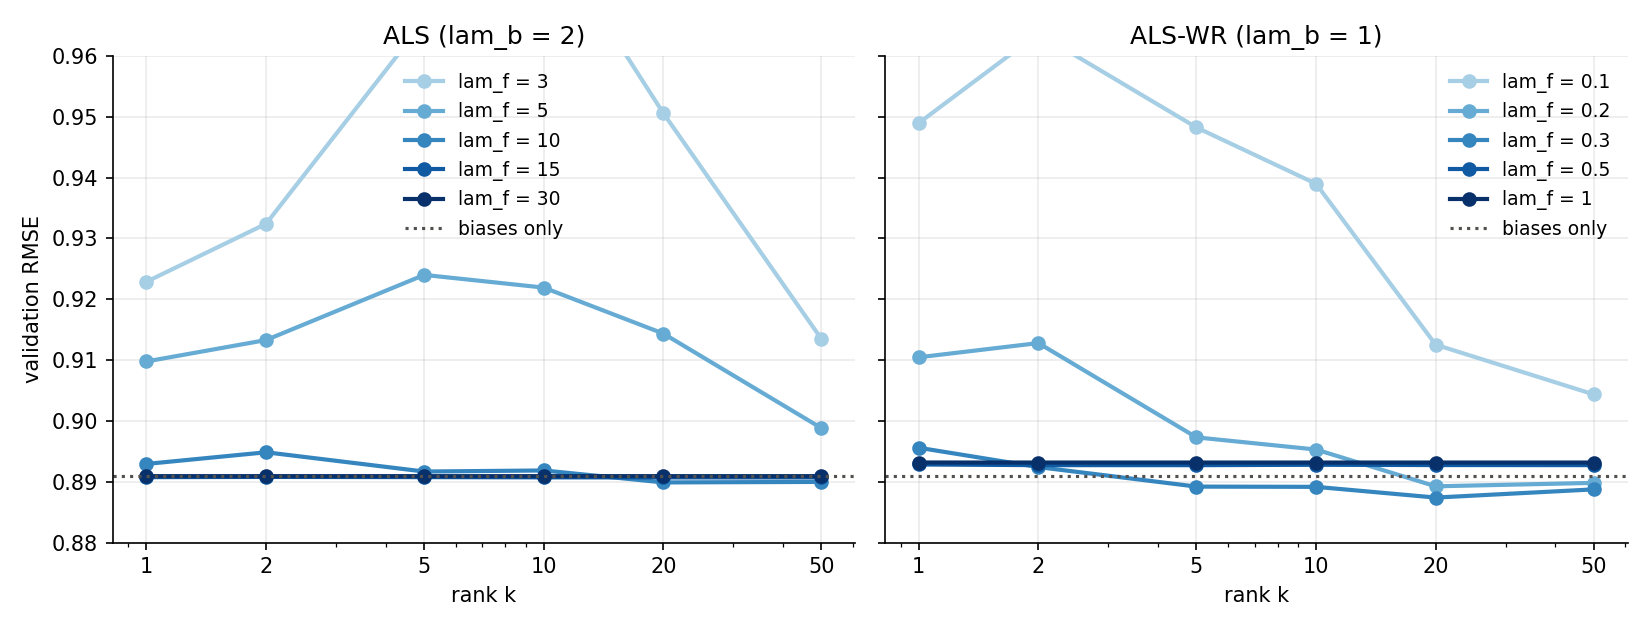
\includegraphics[width=0.8\linewidth]{mf_rank.png}
\caption{Haut : RMSE d'entraînement (pointillés) et de validation (traits pleins)
au fil des itérations, sans régularisation (orange) et avec (bleu). Bas : RMSE
de validation selon le rang $k$ pour plusieurs $\lambda_f$ ; la ligne pointillée
correspond aux biais seuls.}
\label{fig:mf}
\end{figure}

%-----------------------------------------------------------------------------
\begin{etape}{Étape 3 --- Approches alternatives \hfill \textcolor{ok}{fait}}
\textbf{Objectif :} comparer des familles de méthodes qui exploitent une
information différente.

\begin{itemize}
  \item \textbf{Soft-Impute} (complétion par norme nucléaire). On cherche une
        matrice de faible rang \emph{sans fixer le rang} :
        $\min_Z \tfrac12 \sum_{\text{obs.}} (r_{ui} - z_{ui})^2 + \tau \|Z\|_*$.
        On itère : remplir les trous avec la prédiction courante, faire une SVD,
        retirer $\tau$ à chaque valeur singulière (et mettre à 0 celles qui
        deviennent négatives). Meilleur réglage : $\tau = 10$, RMSE $0{,}8716$
        en $4{,}7$\,s.
  \item \textbf{$k$ plus proches voisins sur les films} (vu en cours). Pour
        prédire $r_{ui}$, on regarde les films les plus similaires à $i$ que
        $u$ a notés, avec une similarité de Pearson sur les résidus des biais,
        \emph{rétrécie} quand deux films ont peu de notes en commun :
        $s_{ij} \leftarrow s_{ij}\,\frac{n_{ij}}{n_{ij} + 100}$. La formule du
        cours, normalisée par $\sum |s_{ij}|$, surcorrige quand il y a peu de
        voisins ; ajouter une petite constante $\beta = 0{,}2$ au dénominateur
        règle le problème. RMSE $0{,}8705$ : meilleur modèle seul.
  \item \textbf{Biais guidés par les métadonnées.} Le biais d'un film est tiré
        vers une valeur prédite par ses genres, sa décennie et sa popularité,
        plutôt que vers 0. Le gain global est petit ($0{,}8736$) mais ciblé :
        c'est le seul modèle qui améliore les films à 1--2 notes.
\end{itemize}
\end{etape}

%-----------------------------------------------------------------------------
\begin{etape}{Étape 4 --- Mélange de modèles \hfill \textcolor{ok}{fait}}
\textbf{Objectif :} combiner des modèles qui se trompent différemment.

\textbf{Méthode :} chaque modèle est entraîné sur les $90\,\%$ de train ; une
régression ridge apprend, sur la validation, les poids de la combinaison
$\rhat_{ui} = w_0 + \sum_m w_m\, \rhat^{(m)}_{ui}$. Les modèles sont ensuite
réentraînés sur tout le train et combinés avec ces poids.

\textbf{Résultat :} RMSE $0{,}8683$, le meilleur score à ce jour. La
figure~\ref{fig:pop} montre pourquoi : le $k$NN et Soft-Impute gagnent sur les
films populaires, les biais guidés par les genres sur les films rares.
\end{etape}

\begin{figure}[H]
\centering
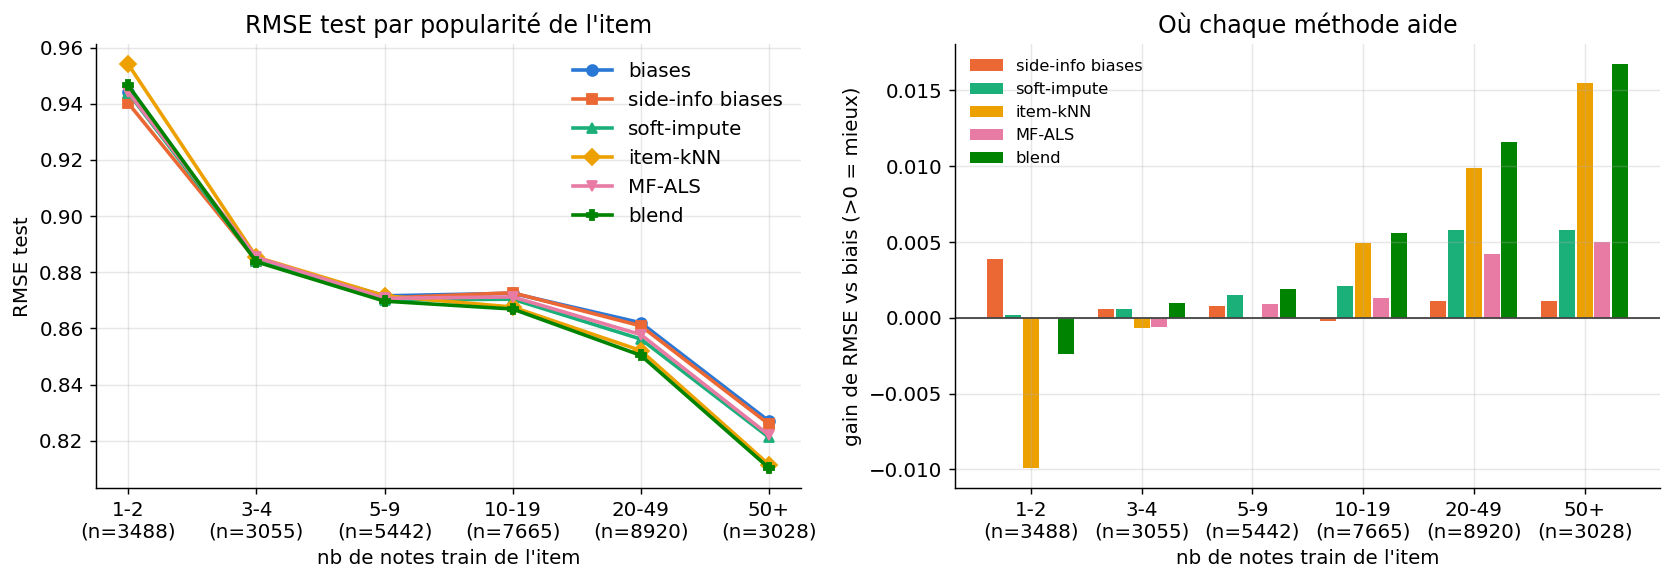
\includegraphics[width=\linewidth]{alt/rmse_by_popularity.png}
\caption{RMSE de test selon le nombre de notes du film en train (gauche) et gain
de chaque méthode par rapport aux biais seuls (droite).}
\label{fig:pop}
\end{figure}

%-----------------------------------------------------------------------------
\begin{etape}{Étape 5 --- Méthodes de l'état de l'art \hfill \textcolor{warm}{à faire}}
\textbf{Objectif :} tester les deux pistes que la littérature désigne comme les
plus prometteuses sur de petites données creuses (section~\ref{sec:sota}).

\begin{itemize}
  \item \textbf{Factorisation bayésienne (BPMF / factorization machine par MCMC).}
        Au lieu d'un seul jeu de facteurs, on moyenne les prédictions de
        nombreux échantillons de la loi a posteriori : la régularisation est
        apprise, plus besoin de régler $\lambda$. Sur MovieLens-10M, c'est
        l'une des meilleures méthodes connues~\cite{rendle2019}. Variante
        enrichie : ajouter au modèle l'ensemble des films notés par chaque
        utilisateur (SVD++) et les genres.
  \item \textbf{AutoRec}~\cite{autorec}. Un auto-encodeur à une couche cachée
        (500 neurones) reçoit le vecteur des notes d'un film et apprend à le
        reconstruire ; la perte ne porte que sur les notes observées. C'est la
        méthode profonde la plus simple et la plus efficace en RMSE ; on la
        prévoit surtout comme membre supplémentaire du mélange.
\end{itemize}
\end{etape}

%-----------------------------------------------------------------------------
\begin{etape}{Étape 6 --- Version finale pour la plateforme \hfill \textcolor{warm}{à faire}}
\begin{itemize}
  \item Brancher le mélange dans \texttt{generate.py} et vérifier le temps sur
        4 threads (objectif : moins de 300\,s, marge large sous 1200\,s).
  \item Décider si \texttt{namesngenre.npy} doit être versionné dans le dépôt :
        la plateforme ne garantit pas sa présence.
  \item Ne \textbf{pas} arrondir les prédictions : l'accuracy ne change pas
        (la plateforme arrondit déjà) et la RMSE se dégrade d'environ $0{,}012$.
  \item Contrôle de robustesse : validation croisée à 5 plis sur train + test
        pour vérifier que les hyperparamètres restent bons avec deux fois plus
        de données.
\end{itemize}
\end{etape}

%=============================================================================
\section{Résultats à ce jour}
%=============================================================================

\begin{table}[H]
\centering
\small
\setlength{\tabcolsep}{4pt}
\begin{tabular}{@{}lccccr@{}}
\toprule
\textbf{Méthode} & \textbf{RMSE valid.} & \textbf{RMSE test} & \textbf{Acc.\ test}
  & \textbf{RMSE rares} & \textbf{Temps (s)} \\
\midrule
Moyenne globale        & ---    & 1,0369 & 0,129 & ---    & 0,00 \\
Biais ($\lambda=2$)    & 0,8909 & 0,8746 & 0,244 & 0,9168 & 0,01 \\
Biais + métadonnées    & 0,8889 & 0,8736 & 0,246 & \textbf{0,9145} & 0,04 \\
Factorisation SGD ($k=20$) & 0,8932 & 0,8775 & 0,243 & ---    & 0,5 \\
Factorisation ALS ($k=20$) & 0,8899 & 0,8725 & 0,247 & ---    & 1,5 \\
Soft-Impute ($\tau=10$) & 0,8892 & 0,8716 & 0,248 & 0,9165 & 4,67 \\
$k$NN films ($k=40$)   & 0,8848 & 0,8705 & \textbf{0,249} & 0,9226 & 1,05 \\
\midrule
\textbf{Mélange ridge} & \textbf{0,8837} & \textbf{0,8683} & 0,247 & 0,9177 & 7,73 \\
\bottomrule
\end{tabular}
\caption{Entraînement sur train, score sur test. \og Films rares \fg{} : notes de
test des films ayant moins de 5 notes en train (6\,543 notes).}
\label{tab:res}
\end{table}

Pour situer ces chiffres : les meilleures références du classement de la
plateforme sont autour de $0{,}80$--$0{,}82$, mais elles disposent de deux fois
plus de notes en entrée. L'écart entre méthodes est faible (moins de $0{,}01$)
parce que les biais captent presque tout le signal disponible : c'est un
résultat en soi, à expliquer dans la présentation.

%=============================================================================
\section{État de l'art}
\label{sec:sota}
%=============================================================================

\subsection{Méthodes classiques}

\begin{itemize}
  \item \textbf{Biais et factorisation}~\cite{koren2009} : la référence du
        Netflix Prize. SVD++~\cite{koren2008} ajoute pour chaque utilisateur
        l'information implicite \og quels films il a notés \fg{}.
  \item \textbf{Complétion convexe} : Soft-Impute~\cite{softimpute}, et sa
        version pondérée pour un échantillonnage non uniforme~\cite{srebro2010}.
  \item \textbf{Approches bayésiennes} : PMF~\cite{pmf} puis BPMF par
        échantillonnage de Gibbs~\cite{bpmf}. Rendle et al.~\cite{rendle2019}
        montrent qu'une MF bayésienne bien réglée bat toutes les méthodes
        profondes publiées sur MovieLens-10M.
  \item \textbf{Voisinage} : $k$NN avec similarités rétrécies et biais
        (KNNBaseline), plus robuste que le $k$NN brut sur données creuses.
\end{itemize}

\subsection{Méthodes profondes}

\begin{table}[H]
\centering
\begin{tabular}{@{}llccl@{}}
\toprule
\textbf{Méthode} & \textbf{Référence} & \textbf{ML-100K} & \textbf{ML-1M} & \textbf{Pour nous} \\
\midrule
I-AutoRec   & Sedhain et al., 2015~\cite{autorec}   & 0,895 & 0,831 & oui, simple \\
Sparse FC   & Muller et al., 2018~\cite{sparsefc}   & 0,890 & 0,824 & variante d'AutoRec \\
GLocal-K    & Han et al., 2021~\cite{glocalk}       & 0,889 & 0,822 & si le temps le permet \\
GC-MC       & van den Berg et al., 2017~\cite{gcmc} & 0,905 & 0,832 & non \\
IGMC        & Zhang \& Chen, 2020~\cite{igmc}       & 0,905 & 0,857 & non (trop lent sur CPU) \\
NCF         & He et al., 2017~\cite{ncf}            & ---   & ---   & non (feedback implicite) \\
\bottomrule
\end{tabular}
\caption{RMSE publiées. Nos données sont 2 à 3 fois plus creuses que ML-100K.}
\end{table}

\begin{retenir}
Sur des données aussi creuses que les nôtres, les méthodes profondes perdent
une grande partie de leur avance~\cite{glocalk}, et une factorisation
bayésienne bien réglée reste un adversaire redoutable~\cite{rendle2019,rendle2020}.
Leur intérêt principal ici est d'apporter de la diversité au mélange.
\end{retenir}

%=============================================================================
\section{Présentation du 15 octobre et rapport}
%=============================================================================

\subsection{Slides : 5 minutes, 6 diapositives}

La présentation préliminaire doit énoncer le problème, comparer les approches,
dire ce qui est fait, décrire le protocole et montrer de premiers résultats. Pas
de rappel de cours, des équations composées en \LaTeX{}, pas de captures
d'écran.

\begin{table}[H]
\centering
\begin{tabular}{@{}clp{8.2cm}r@{}}
\toprule
\textbf{\#} & \textbf{Titre} & \textbf{Contenu} & \textbf{Durée} \\
\midrule
1 & Le problème & Matrice 610\,$\times$\,4980, 1\,\% observé, RMSE ; question : \emph{que peut-on apprendre au-delà des biais ?} & 30\,s \\
2 & Les données & Longue traîne, 3 notes par film en médiane, spectre vs bruit & 45\,s \\
3 & Protocole & Validation 10\,\%, test jamais utilisé pour régler ; local vs plateforme & 40\,s \\
4 & Méthodes & Biais, MF (ALS/SGD), Soft-Impute, $k$NN, mélange : une équation chacune & 75\,s \\
5 & Résultats & Tableau~\ref{tab:res} et figure~\ref{fig:pop} & 60\,s \\
6 & Suite & MF bayésienne, AutoRec, version plateforme & 30\,s \\
\bottomrule
\end{tabular}
\end{table}

\subsection{Rapport : 5 pages}

Même fil que les slides, en développant ce que l'oral ne permet pas :
réglage des hyperparamètres (courbes), coût de calcul, échecs instructifs (la
formule $k$NN du cours qui surcorrige, l'arrondi qui dégrade la RMSE), et une
séparation nette entre observations, hypothèses et limites. Chaque méthode
renvoie à son fichier source dans \texttt{src/}.

%=============================================================================
\begin{thebibliography}{99}
\small
\bibitem{koren2009} Y.~Koren, R.~Bell, C.~Volinsky. \emph{Matrix Factorization
  Techniques for Recommender Systems}. IEEE Computer, 2009.
\bibitem{koren2008} Y.~Koren. \emph{Factorization Meets the Neighborhood: a
  Multifaceted Collaborative Filtering Model}. KDD, 2008.
\bibitem{softimpute} R.~Mazumder, T.~Hastie, R.~Tibshirani. \emph{Spectral
  Regularization Algorithms for Learning Large Incomplete Matrices}. JMLR, 2010.
\bibitem{srebro2010} R.~Salakhutdinov, N.~Srebro. \emph{Collaborative Filtering in
  a Non-Uniform World: Learning with the Weighted Trace Norm}. NeurIPS, 2010.
\bibitem{pmf} R.~Salakhutdinov, A.~Mnih. \emph{Probabilistic Matrix
  Factorization}. NeurIPS, 2007.
\bibitem{bpmf} R.~Salakhutdinov, A.~Mnih. \emph{Bayesian Probabilistic Matrix
  Factorization using Markov Chain Monte Carlo}. ICML, 2008.
\bibitem{rendle2019} S.~Rendle, L.~Zhang, Y.~Koren. \emph{On the Difficulty of
  Evaluating Baselines: A Study on Recommender Systems}. arXiv:1905.01395, 2019.
\bibitem{rendle2020} S.~Rendle, W.~Krichene, L.~Zhang, J.~Anderson. \emph{Neural
  Collaborative Filtering vs. Matrix Factorization Revisited}. RecSys, 2020.
\bibitem{autorec} S.~Sedhain, A.~K.~Menon, S.~Sanner, L.~Xie. \emph{AutoRec:
  Autoencoders Meet Collaborative Filtering}. WWW Companion, 2015.
\bibitem{sparsefc} L.~Muller, J.~Martel, G.~Indiveri. \emph{Kernelized Synaptic
  Weight Matrices}. ICML, 2018.
\bibitem{glocalk} S.~C.~Han, T.~Lim, S.~Long, B.~Burgstaller, J.~Poon.
  \emph{GLocal-K: Global and Local Kernels for Recommender Systems}. CIKM, 2021.
\bibitem{gcmc} R.~van den Berg, T.~N.~Kipf, M.~Welling. \emph{Graph Convolutional
  Matrix Completion}. arXiv:1706.02263, 2017.
\bibitem{igmc} M.~Zhang, Y.~Chen. \emph{Inductive Matrix Completion Based on
  Graph Neural Networks}. ICLR, 2020.
\bibitem{ncf} X.~He, L.~Liao, H.~Zhang, L.~Nie, X.~Hu, T.-S.~Chua. \emph{Neural
  Collaborative Filtering}. WWW, 2017.
\end{thebibliography}

\end{document}
